% Smart Plant Monitoring System - final report (LNCS, max. 6 pages)
% Compile on Overleaf: upload this file and the figures/ folder.
% llncs.cls is included in TeX Live/Overleaf (or download it from the
% Springer LNCS guidelines page and put it next to this file).
\documentclass[runningheads]{llncs}
\usepackage[T1]{fontenc}
\usepackage{graphicx}
\usepackage{booktabs}
\usepackage{siunitx}
\usepackage{tikz}
\usetikzlibrary{positioning,arrows.meta}
\usepackage{url}
\usepackage[hidelinks]{hyperref}
\sisetup{group-minimum-digits=4}

\begin{document}

\title{Smart Plant Monitoring with an Always-On ESP32 and an On-Demand Raspberry Pi}
\titlerunning{Energy-Efficient Smart Plant Monitoring}
\author{Manuel Gon\c{c}alves \and Nik Kopi}
\authorrunning{M. Gon\c{c}alves and N. Kopi}
\institute{Programming of Energy-Constrained Devices, University of Ljubljana, Faculty of Computer and Information Science\\
Code and measurements: \url{https://github.com/ELITE-Salty/PECD} (folder \texttt{FINAL\_Smart\_Plant\_NM})}

\maketitle

\begin{abstract}
We built a plant monitor that checks soil moisture, air temperature and humidity, raises buzzer alarms and looks at the plant with a camera. A low-power ESP32 runs all the time and wakes a Raspberry Pi only when a photo is needed. We measured every part with a Monsoon power monitor. The unoptimised system (ESP32 always awake, Pi always on) needs about \SI{126}{kJ} per day; our design, with deep sleep, an adaptive sensing interval and event-driven photos, needs about \SI{4.4}{kJ} per day in a simulated three-day scenario, almost 30 times less, and still detects a dry pot within about a minute.
\keywords{ESP32 \and Raspberry Pi \and adaptive sampling \and sleep modes}
\end{abstract}

% ---------------------------------------------------------------------------
\section{Introduction}

The task was to monitor a plant from our greenhouse kit, a dwarf sunflower (\emph{Helianthus annuus} `Sunspot'), with a soil moisture sensor, a DHT11 and a camera, as energy-efficiently as possible. Our measurements show how different the two boards are: the ESP32 DevKit uses \SI{219}{mW} awake and \SI{45}{mW} in deep sleep, while the Raspberry Pi 3B uses \SI{1.24}{W} doing nothing and \SI{200}{J} just to boot. Most of our work was therefore deciding \emph{when} each device should be awake.

\noindent\textbf{Who did what.} \emph{Manuel} was responsible for the ESP32: firmware for the soil sensor, DHT11 and buzzer, alarm rules, event log, soil calibration, adaptive sampling, and the ESP32 energy measurements with the Monsoon. \emph{Nik} was responsible for the Raspberry Pi: Pi and camera set-up, the two-stage vision pipeline, the UART protocol with the ESP32, and the wake/power-off cycle. The test scenario, the measurements and the report were done together. We used AI assistants for code review, plotting scripts and language editing; the measurements and design decisions are our own.

% ---------------------------------------------------------------------------
\section{Design: Why We Built It This Way}

\begin{figure}[t]
\centering
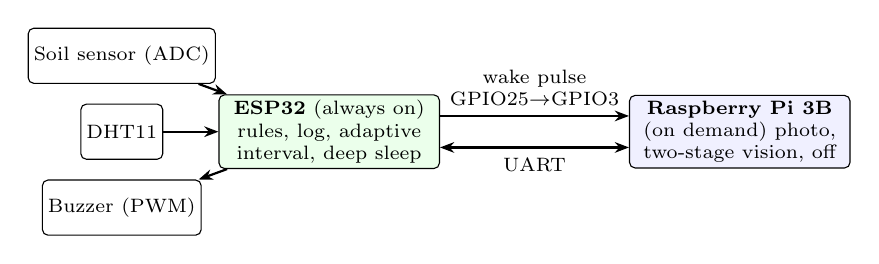
\begin{tikzpicture}[font=\scriptsize, node distance=2.5mm and 7mm,
  box/.style={draw, rounded corners=2pt, align=center, minimum height=7mm, inner sep=2pt},
  arr/.style={-{Stealth[length=1.8mm]}, thick}]
\node[box] (soil) {Soil sensor (ADC)};
\node[box, below=of soil] (dht) {DHT11};
\node[box, below=of dht] (buz) {Buzzer (PWM)};
\node[box, fill=green!8, right=of dht, minimum width=28mm] (esp) {\textbf{ESP32} (always on)\\rules, log, adaptive\\interval, deep sleep};
\node[box, fill=blue!6, right=24mm of esp, minimum width=28mm] (pi) {\textbf{Raspberry Pi 3B}\\(on demand) photo,\\two-stage vision, off};
\draw[arr] (soil) -- (esp); \draw[arr] (dht) -- (esp); \draw[arr] (esp) -- (buz);
\draw[arr] ([yshift=2mm]esp.east) -- node[above, align=center]{wake pulse\\GPIO25$\to$GPIO3} ([yshift=2mm]pi.west);
\draw[arr, {Stealth[length=1.8mm]}-{Stealth[length=1.8mm]}] ([yshift=-2mm]esp.east) -- node[below]{UART} ([yshift=-2mm]pi.west);
\end{tikzpicture}
\caption{Architecture: the ESP32 senses all the time; the Pi is booted only for a photo.}
\label{fig:arch}
\end{figure}

\noindent\textbf{Hierarchical sensing.} Soil and air readings are cheap, but the camera and models need the Pi, and keeping it on all day costs $\SI{1.24}{W}\times\SI{24}{h}\approx\SI{107}{kJ}$, about 27 times more than the ESP32 board in deep sleep. Yellowing develops over days, so one photo a day, plus one when something goes wrong, is enough. We therefore split the system as in Fig.~\ref{fig:arch}, similar to multi-tier power management on mobile devices~\cite{turducken}; a low pulse on GPIO3 boots a halted Pi.

\noindent\textbf{The baseline.} We compare against the system as it first worked after the labs, with no energy optimisation: (a) ESP32 firmware \texttt{unoptimised.c}, always awake, reading both sensors every $\approx$\SI{2.5}{s} and waiting up to \SI{2}{s} for a UART reply from the Pi in every cycle; (b) the Pi left on so it can take photos at any time. We measured both; Sect.~\ref{sec:compare} also compares with a fixed-interval alternative.

\noindent\textbf{Rules.} Alarms come from \texttt{configuration.txt} in the assignment's format. For the sunflower: 1 beep if humidity $>85\%$ (fungal diseases), 2 if temperature $<\SI{10}{\celsius}$ (growth stops), 3 if soil $<300/1000$, 5 if temperature $>\SI{35}{\celsius}$ (heat stress)~\cite{schneiter,berglund}; 4 beeps are the vision alarm. A rule beeps only when it becomes true, so a dry pot does not beep every minute.

% ---------------------------------------------------------------------------
\section{Implementation: How We Did It}

\noindent\textbf{ESP32 firmware} (C, ESP-IDF). The soil sensor uses the one-shot ADC (12 bit), the DHT11 the \texttt{esp-idf-lib} driver. Our two-point calibration gave 0 in air and $\approx$2350 raw in wet soil (noise $\pm 15$); raw 2560 (saturation) maps to 1000, so wet soil reads $\approx 920$. Every reading and buzzer action is appended to \texttt{events\_log.txt} on SPIFFS (time since power-on, as there is no clock). We kept variants so that each optimisation could be measured alone: \texttt{unoptimised.c} (baseline), \texttt{optimised.c} (same work, then \SI{10}{s} light or deep sleep) and the final \texttt{adaptive.c}. The final version deep-sleeps between readings, keeps its state in RTC memory, and listens on UART only after it has woken the Pi, until the Pi has fetched the log (at most \SI{5}{min}).

\subsection{How the sensing interval is selected}\label{sec:interval}
The logic is a small C header compiled both into the firmware and into a PC test, so the simulation in Sect.~\ref{sec:scenario} runs exactly the firmware code.
(1)~The interval starts at \SI{60}{s} and doubles after every reading without change, up to \SI{900}{s} (60, 120, 240, 480, 900).
(2)~``Without change'' means smaller than the sensor noise: 20/1000 for soil (we measured about $\pm 6$), \SI{1}{\celsius} and 3\,\% for the DHT11 (its resolution and jitter), so noise never resets the interval.
(3)~A real change, or a value close to a rule threshold (soil $\pm 50$, \SI{\pm 2}{\celsius}, $\pm 5\%$), resets it to \SI{60}{s}, so the system is fastest exactly when an alarm is about to happen.

The bounds come from our energy model and from the plant. Above \SI{60}{s} the ESP32 board is already within about 6\,\% of its sleep floor (Fig.~\ref{fig:interval}), and one minute is a negligible delay for a plant. The upper bound, \SI{15}{min}, limits the delay for sudden events such as an open window; soil dries over hours. The idea is a much simpler version of~\cite{alippi}.

\noindent\textbf{When to take a photo.} One Pi wake costs about \SI{300}{J} (boot \SI{200}{J} plus photo, vision and shutdown, rounded up), as much as \SI{1.9}{h} of the ESP32 board in deep sleep. The Pi is woken at installation, every \SI{24}{h}, and when an alarm starts, but at most every \SI{6}{h}. A first version also reacted to large soil changes, but in the scenario normal drying triggered it almost daily, so we removed it.

\noindent\textbf{Raspberry Pi and vision.} After a wake the Pi takes a photo (IMX219), runs the vision, sends \texttt{BEEP 4} if the plant looks unhealthy, downloads the ESP32 log and powers off. The vision has two stages: the small U\textsuperscript{2}-Net-p model (\SI{4.6}{MB})~\cite{u2net} separates the plant from the background and a colour rule compares green and yellow/brown area; only if this is uncertain does a MobileNetV3 classifier (\SI{17}{MB}, 15 PlantVillage classes)~\cite{mobilenetv3,plantvillage} run. Sunflowers are not among its classes, so for our plant the pipeline stops at ``uncertain'' instead of giving a confident wrong answer. Both run with ONNX Runtime.

% ---------------------------------------------------------------------------
\section{Evaluation}

\noindent\textbf{Set-up.} Monsoon power monitor at \SI{5.0}{V}, \SI{5}{kHz}, powering the whole board (ESP32 DevKit with USB chip, regulator, LED and both sensors; or Pi 3B with camera). We decoded the \texttt{.pt5} files with our own script. ESP32 baseline: six \SI{5}{min} runs; sleep variants: one run each; Pi: two \SI{10}{min} runs.

\begin{figure}[t]
\centering
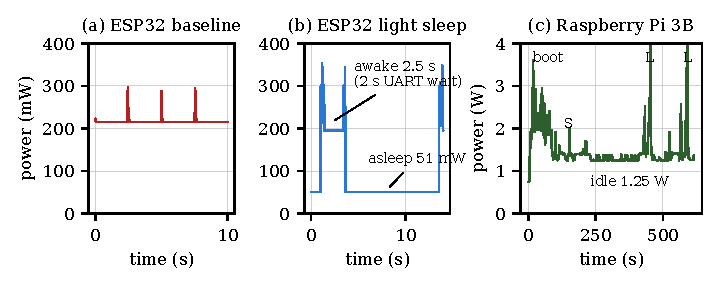
\includegraphics[width=\textwidth]{figures/power_traces.pdf}
\caption{Measured power. (a) Baseline ESP32 (spikes: sensors and log). (b) Light-sleep firmware, one cycle. (c) Pi 3B: boot, idle, small (S) and large (L) model.}
\label{fig:traces}
\end{figure}


\noindent\textbf{Components.} Fig.~\ref{fig:traces} shows the measured traces; two results shaped the design. In the baseline, 97--99\,\% of the ESP32 energy is spent waiting; reading the sensors is almost free. (The cost per cycle grew from 4 to \SI{15}{mJ} between runs; we think appending to a growing log file in flash takes longer, but did not test it separately.) A sensing cycle costs only 4--\SI{15}{mJ}, but the buzzer is expensive: one \SI{5}{s} tone (\SI{0.56}{J}) equals 40--130 sensing cycles, so alarms use short \SI{200}{ms} beeps. On the Pi one run of the large model costs 17--\SI{19}{J} against 1--\SI{5}{J} for the small one, which justifies the two stages, but both are small next to booting or one hour of idling (\SI{4.5}{kJ}). Sleeping \SI{10}{s} between readings lowered the ESP32 from \SI{219}{mW} to \SI{84}{mW} with both sleep modes; at the same reading rate it would use $\approx$\SI{190}{mW} awake, a saving of about 55\,\%. The remaining 45--\SI{51}{mW} is mostly the DevKit (USB chip, regulator, LED), not the ESP32 chip.

\noindent\textbf{Energy model.} We could not record the final firmware before the deadline, so we model it from the measured parts: sleep power $P_s$, awake power $P_a$ and awake time $t_a$. For a sleep interval $T$, $P(T)=(P_s T + P_a t_a)/(T+t_a)$. It reproduces the measured averages (83.9 vs.\ \SI{84.0}{mW}; a consistency check, not a validation). Without the UART wait, $t_a=\SI{0.52}{s}$ (light) or \SI{0.89}{s} (deep, includes the reboot).

\begin{figure}[t]
\centering
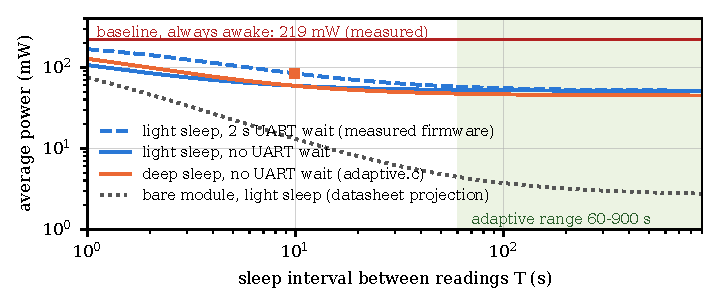
\includegraphics[width=\textwidth]{figures/energy_vs_interval.pdf}
\caption{ESP32 average power vs.\ sleep interval (model from measured parts; markers: measured runs). Dotted: module datasheet sleep current (\SI{0.8}{mA})~\cite{esp32ds} instead of the DevKit.}
\label{fig:interval}
\end{figure}

Fig.~\ref{fig:interval} shows that (1) removing the UART wait matters most at short intervals (84 to \SI{59}{mW} at \SI{10}{s}); (2) deep sleep beats light sleep only above $\approx$\SI{10}{s} because each wake is a reboot, which explains why our \SI{10}{s} runs showed no difference and why \texttt{adaptive.c} uses deep sleep (47 vs.\ \SI{52.5}{mW} at \SI{60}{s}); (3) on the DevKit the curve is flat above \SI{60}{s}, while on a bare module it still falls from 4.4 to \SI{2.8}{mW} between 60 and \SI{900}{s}.

\subsection{Scenario: a sunflower drying out}\label{sec:scenario}
We simulated 3.5 days and ran them through the firmware logic (synthetic values, real decisions, energy from the model). The pot dries from 900 to below 300 (faster by day) and is watered four hours after the alarm; the room follows an 18.5--\SI{24.5}{\celsius} daily cycle; on the second morning a window stays open for an hour (\SI{8}{\celsius}). Noise is similar to what we measured.

\begin{figure}[t]
\centering
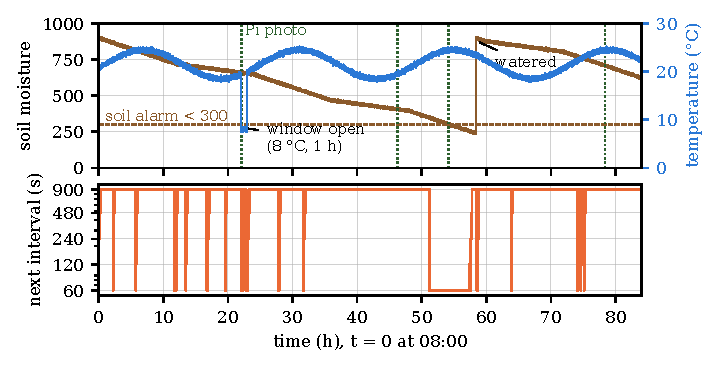
\includegraphics[width=\textwidth]{figures/adaptive_scenario.pdf}
\caption{Simulated scenario. Top: soil, temperature, Pi photos (dotted). Bottom: interval chosen by the firmware logic; it stays at \SI{60}{s} while the soil is near the alarm threshold (hours 51--58).}
\label{fig:scenario}
\end{figure}

\begin{table}[t]
\centering
\caption{Strategies in the scenario: ESP32 energy per day (model, deep sleep), DevKit and bare module; alarm delays from the true threshold crossing.}
\label{tab:strategies}
\setlength{\tabcolsep}{4pt}\small
\begin{tabular}{lrrrrr}
\toprule
strategy & readings/day & DevKit kJ & bare kJ & soil alarm & window\\
\midrule
fixed \SI{2.5}{s} (baseline) & \num{34560} & 18.9 & -- & \SI{51}{s} & \SI{1}{s}\\
fixed \SI{10}{s} & \num{8640} & 5.10 & 1.13 & \SI{54}{s} & \SI{4}{s}\\
fixed \SI{60}{s} & \num{1440} & 4.08 & 0.38 & \SI{92}{s} & \SI{22}{s}\\
fixed \SI{900}{s} & 96 & 3.88 & 0.24 & \SI{703}{s} & \SI{333}{s}\\
\textbf{adaptive 60--\SI{900}{s}} & \textbf{222} & \textbf{3.93} & \textbf{0.29} & \textbf{\SI{70}{s}} & \textbf{\SI{360}{s}}\\
\bottomrule
\end{tabular}
\end{table}

Table~\ref{tab:strategies} shows the trade-off. The adaptive policy takes 85\,\% fewer readings (and log writes) than a fixed \SI{60}{s} interval and finds the dry pot as fast, because it samples every minute near the threshold. Its energy is close to the fixed \SI{900}{s} interval, which finds the dry pot about 10 minutes later. The price is the sudden cold event, found after \SI{6}{min} because the system was in its long interval; sudden changes are always found within \SI{15}{min}, acceptable for a plant. The Pi was woken 5 times: at installation, for the cold and the dry-soil alarms, and twice for the daily photo.

\subsection{Comparison of the whole system}\label{sec:compare}
\begin{table}[t]
\centering
\caption{Energy per day of the whole system. B and C exclude the small, unmeasured standby draw of the halted Pi.}
\label{tab:system}
\setlength{\tabcolsep}{4pt}\small
\begin{tabular}{lrrr}
\toprule
 & ESP32 kJ & Pi kJ & total kJ\\
\midrule
A. Baseline: ESP32 always awake, Pi always on & 18.9 & 107 & 126\\
B. Fixed: \SI{10}{s} light sleep, Pi photo every hour & 7.3 & 7.2 & 14.5\\
C. Ours: adaptive, deep sleep, Pi daily or on alarm & 3.9 & 0.4 & \textbf{4.4}\\
\bottomrule
\end{tabular}
\end{table}

Table~\ref{tab:system} compares the whole system with the baseline (A) and an alternative (B) that already sleeps and switches the Pi off between hourly photos. Ours needs 29 times less energy than A and 3.3 times less than B, mostly thanks to the Pi. On a \SI{7.4}{Wh} battery A would last about 5 hours, B 1.8 days and C about 6 days.

\noindent\textbf{Functional tests and accuracy.} Sensors and rules were checked by hand. In a wake test the Pi was online \SI{74}{s} after the pulse; capture and model routing worked and \texttt{BEEP 4} was acknowledged. A systematic accuracy study (slowly changing conditions, labelled images) is missing; this is the main gap in our evaluation.

% ---------------------------------------------------------------------------
\section{Discussion and Conclusion}
Our main lesson: the cheapest energy is that of a device that is off. We first wanted to optimise the ESP32 code, but sensing costs almost nothing and the Pi dominates. We were also surprised that the \SI{2}{s} UART wait copied from a lab example was 80\,\% of the ESP32's awake time. Limitations: \texttt{adaptive.c} is tested on a PC but not measured on the hardware; the scenario is simulated; the DevKit hides most of the benefit of longer intervals; in our last wake test the UART did not answer after the Pi booted and the auto power-off service was not installed (needs root); the models are not quantised.

% ---------------------------------------------------------------------------
\begin{thebibliography}{9}
\bibitem{alippi} Alippi, C., Anastasi, G., Di~Francesco, M., Roveri, M.: An adaptive sampling algorithm for effective energy management in wireless sensor networks with energy-hungry sensors. IEEE Trans. Instrum. Meas. \textbf{59}(2), 335--344 (2010)
\bibitem{berglund} Berglund, D.R. (ed.): Sunflower Production. NDSU Extension Service A-1331, North Dakota State University (2007)
\bibitem{esp32ds} Espressif Systems: ESP32 Series Datasheet, \url{https://www.espressif.com}
\bibitem{mobilenetv3} Howard, A., et al.: Searching for MobileNetV3. In: Proc. ICCV, pp. 1314--1324 (2019)
\bibitem{plantvillage} Mohanty, S.P., Hughes, D.P., Salath\'e, M.: Using deep learning for image-based plant disease detection. Front. Plant Sci. \textbf{7}, 1419 (2016)
\bibitem{u2net} Qin, X., Zhang, Z., Huang, C., Dehghan, M., Zaiane, O.R., Jagersand, M.: U\textsuperscript{2}-Net: going deeper with nested U-structure for salient object detection. Pattern Recognit. \textbf{106}, 107404 (2020)
\bibitem{schneiter} Schneiter, A.A. (ed.): Sunflower Technology and Production. Agronomy Monograph 35, ASA, CSSA, SSSA, Madison, WI (1997)
\bibitem{turducken} Sorber, J., Banerjee, N., Corner, M.D., Rollins, S.: Turducken: hierarchical power management for mobile devices. In: Proc. MobiSys, pp. 261--274 (2005)
\end{thebibliography}

\end{document}
